\documentclass[tikz]{standalone}

\begin{document}
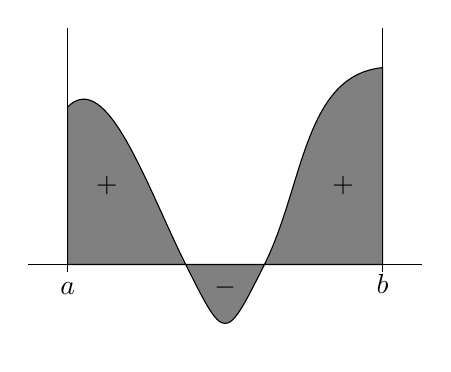
\begin{tikzpicture}
  \draw (-0.5, 0) -- (4.5, 0);
  \draw (0, -0.1) -- (0, 3);
  \draw (4, -0.1) -- (4, 3);

  \node at (0, -0.30) {$a$};
  \node at (4, -0.25) {$b$};
  \draw[fill=gray] (0, 2) ..
    controls +(0.5, 0.5)
    and +(-0.5, 1)
    .. (1.5, 0) -- (0, 0)
    -- cycle;
  \node at (0.5, 1) {$+$};
  \draw[fill=gray]
    (1.5, 0) .. controls
    +(0.5, -1) and
    +(-0.5, -1) ..
    (2.5, 0)
    -- (1.5, 0);
  \node at (2, -0.3) {$-$};
  \draw[fill=gray] (2.5, 0) ..
    controls +(0.5, 1)
    and +(-1, -0.1)
    .. (4, 2.5) -- 
    (4, 0) -- (2.5, 0);
  \node at (3.5, 1) {$+$};


\end{tikzpicture}
\end{document}
